%-------------------------
% Resume in Latex
% Author : Gennadii Chursov
% Based off of: https://github.com/sb2nov/resume and https://www.overleaf.com/latex/templates/jakes-resume/syzfjbzwjncs
% License : MIT
%------------------------

\documentclass[letterpaper,11pt]{article}
\usepackage{enumitem}
\usepackage{latexsym}
\usepackage[empty]{fullpage}
\usepackage{titlesec}
\usepackage{marvosym}
\usepackage[usenames,dvipsnames]{color}
\usepackage{verbatim}
\usepackage{enumitem}
\usepackage[hidelinks]{hyperref}
\usepackage{fancyhdr}
\usepackage[english]{babel}
\usepackage{tabularx}
\input{glyphtounicode}
\usepackage{siunitx}
\usepackage{hyperref} % Add this line to the preamble of your document
\usepackage{graphicx} % For including images
\usepackage{tikz} % For circular image cropping
\usepackage{fontawesome} % For icons


%----------FONT OPTIONS----------
% sans-serif
% \usepackage[sfdefault]{FiraSans}
% \usepackage[sfdefault]{roboto}
% \usepackage[sfdefault]{noto-sans}
% \usepackage[default]{sourcesanspro}

% serif
% \usepackage{CormorantGaramond}
% \usepackage{charter}


\pagestyle{fancy}
\fancyhf{} % clear all header and footer fields
\fancyfoot{}
\renewcommand{\headrulewidth}{0pt}
\renewcommand{\footrulewidth}{0pt}

% Adjust margins
\addtolength{\oddsidemargin}{-0.5in}
\addtolength{\evensidemargin}{-0.5in}
\addtolength{\textwidth}{1in}
\addtolength{\topmargin}{-.5in}
\addtolength{\textheight}{1.0in}

\urlstyle{same}

\raggedbottom
\raggedright
\setlength{\tabcolsep}{0in}

% Sections formatting
\titleformat{\section}{
  \vspace{-4pt}\scshape\raggedright\large
}{}{0em}{}[\color{black}\titlerule \vspace{-5pt}]

% Ensure that generate pdf is machine readable/ATS parsable
\pdfgentounicode=1

%-------------------------
% Custom commands
\newcommand{\resumeItem}[1]{
  \item\small{
    {#1 \vspace{-2pt}}
  }
}

\newcommand{\resumeSubheading}[4]{
  \vspace{-2pt}\item
    \begin{tabular*}{0.97\textwidth}[t]{l@{\extracolsep{\fill}}r}
      \textbf{#1} & #2 \\
      \textit{\small#3} & \textit{\small #4} \\
    \end{tabular*}\vspace{-7pt}
}

\newcommand{\resumeSubSubheading}[2]{
    \item
    \begin{tabular*}{0.97\textwidth}{l@{\extracolsep{\fill}}r}
      \textit{\small#1} & \textit{\small #2} \\
    \end{tabular*}\vspace{-7pt}
}

\newcommand{\resumeProjectHeading}[2]{
    \item
    \begin{tabular*}{0.97\textwidth}{l@{\extracolsep{\fill}}r}
      \small#1 & #2 \\
    \end{tabular*}\vspace{-7pt}
}

\newcommand{\resumeSubItem}[1]{\resumeItem{#1}\vspace{-4pt}}

\renewcommand\labelitemii{$\vcenter{\hbox{\tiny$\bullet$}}$}

\newcommand{\resumeSubHeadingListStart}{\begin{itemize}[leftmargin=0.15in, label={}]}
\newcommand{\resumeSubHeadingListEnd}{\end{itemize}}
\newcommand{\resumeItemListStart}{\begin{itemize}}
\newcommand{\resumeItemListEnd}{\end{itemize}\vspace{-5pt}}

%-------------------------------------------
%%%%%%  RESUME STARTS HERE  %%%%%%%%%%%%%%%%%%%%%%%%%%%%


\begin{document}

%----------HEADING----------

\noindent
\begin{minipage}[c]{0.05\textwidth}
\-\
\end{minipage}
\begin{minipage}[c]{0.2\textwidth}
\begin{tikzpicture}
    \clip (0,0) circle (1.75cm);
    \node at (0,-0.5) {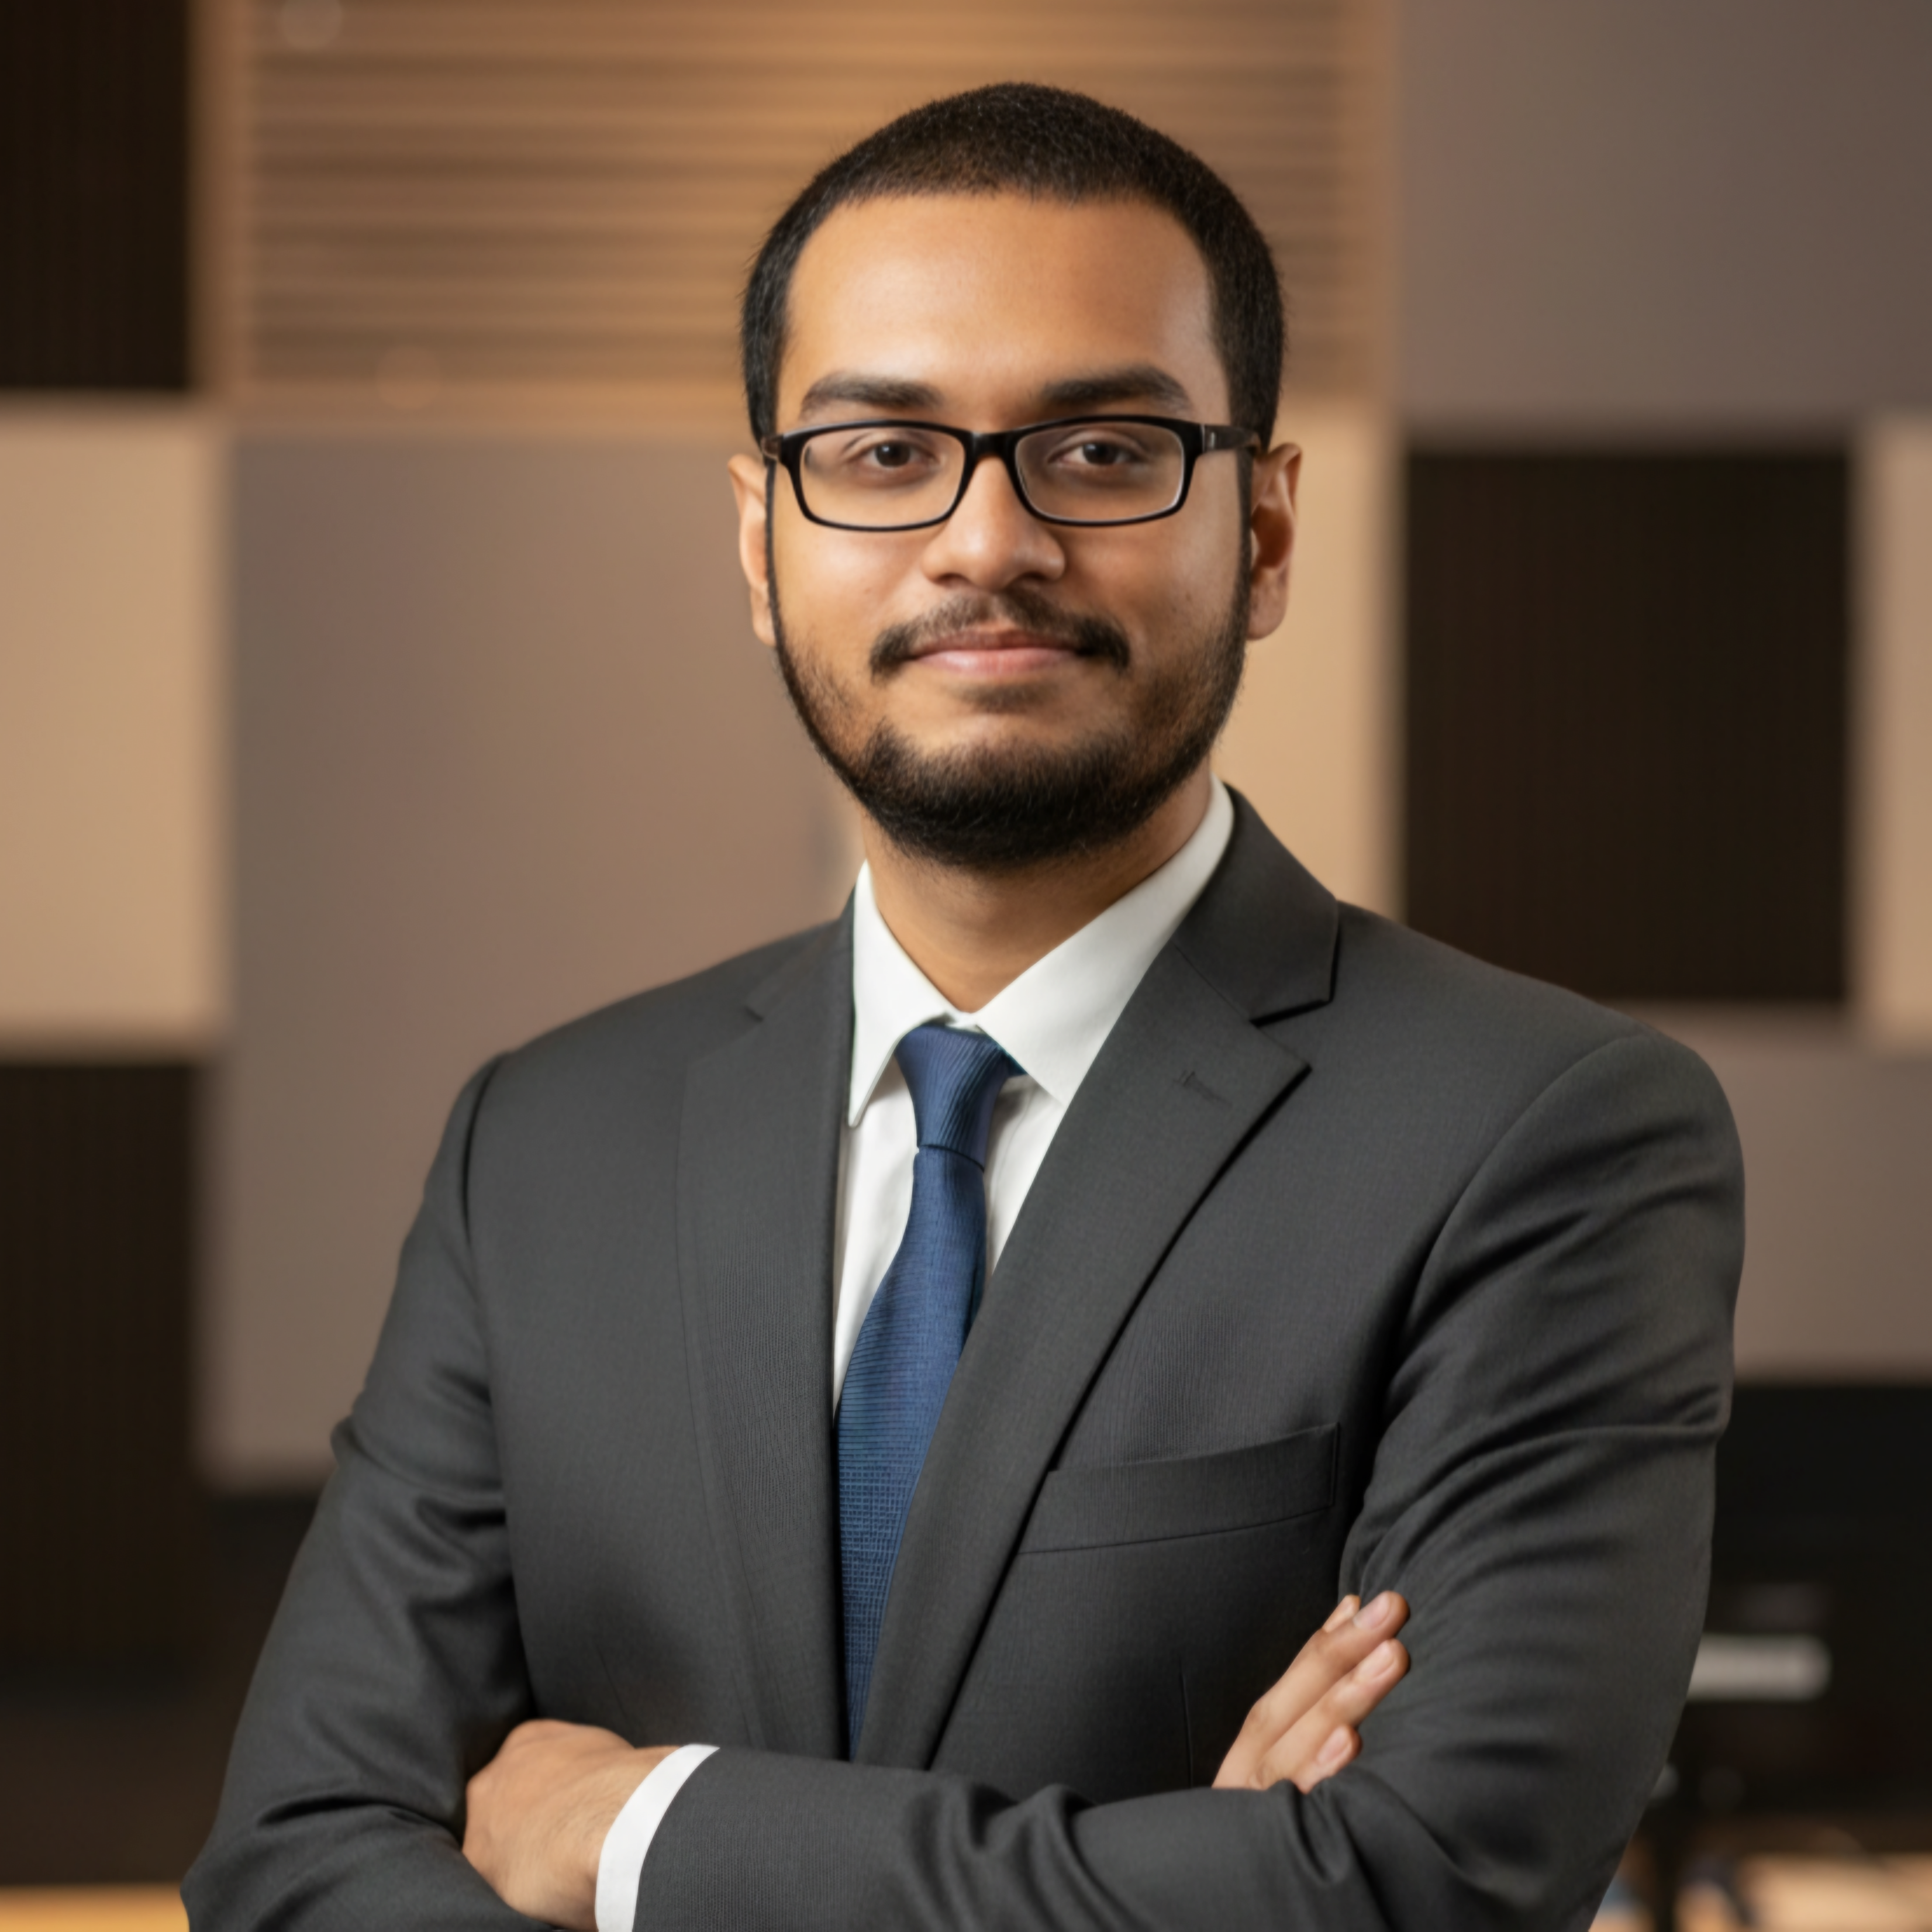
\includegraphics[width = 4cm]{formal2.jpg}}; 
    % if necessary the picture may be moved by changing the at (coordinates)
    % width defines the 'zoom' of the picture
\end{tikzpicture}
\hfill\vline\hfill
\end{minipage}
\begin{minipage}[c]{0.3\textwidth}
    \makebox[\textwidth][l]{\textbf{\Huge \scshape{Md Sakib Sadman Badhon}}} \\[0.4em]
    {\large\textit{Mohammadpur, Dhaka}} \\[0.8em]
    \mbox{{\footnotesize\faPhone}\hspace*{0.13cm}\small +8801838214970} \\
    \mbox{{\footnotesize\faEnvelope}\hspace*{0.13cm}\small \href{mailto:badhon495@gmail.com}{badhon495@gmail.com}} \\
    \mbox{{\footnotesize\faGlobe}\hspace*{0.13cm}\small \href{https://badhon495.github.io/}{badhon495.github.io}} \hspace{0.2cm}
    \mbox{{\footnotesize\faLinkedin}\hspace*{0.13cm}\small \href{https://www.linkedin.com/in/badhon495/}{badhon495}} \hspace{0.2cm}
    \mbox{{\footnotesize\faGithub}\hspace*{0.13cm}\small \href{https://github.com/badhon495}{badhon495}}
\end{minipage}

\vspace{10pt}

\section{Summary}
A Computer Science student with \textbf{strong foundation in software development, system operations, and open-source contributions}. Demonstrated expertise in full-stack web development, automation, and cybersecurity through academic projects and professional experience. Proven ability to deliver practical solutions while maintaining excellence in academics.

%-----------EDUCATION-----------
\section{Education}
\resumeSubHeadingListStart
\resumeSubheading
{Bachelor of Science in Computer Science}{CGPA 3.74/4.00}
{\href{https://www.bracu.ac.bd/}{BRAC University}} {Jan 2022 - Jan 2026}
\resumeItemListStart
\resumeItem{Recognized on the \href{https://www.bracu.ac.bd/academics/policies-and-procedures/academic-standings-and-honors}{\textbf{Vice Chancellor's List, Dean's List}}, and awarded the \href{https://www.bracu.ac.bd/admissions/international-applicants/scholarship-financial-aid}{\textbf{Merit Scholarship}} Based on BRAC University Academic Results across \textbf{multiple semesters} for academic excellence.}
\resumeItemListEnd

\resumeSubheading
{Higher Secondary Certificate, Science}{CGPA 4.58/5.00}
{\href{https://mgcdhaka.edu.bd/}{Mohammadpur Government College}}{2019}

\resumeSubheading
{Secondary School Certificate, Science}{CGPA 5.00/5.00}
{\href{https://www.mghs.edu.bd/}{Mohammadpur Government High School}}{2017}

\resumeSubHeadingListEnd



%-----------PROJECTS-----------
\section{Projects}
\resumeSubHeadingListStart

  \resumeProjectHeading
    {\textbf{\href{https://github.com/badhon495/ParkIt}{ParkIt}} $|$ \emph{Laravel, PostgreSQL} $|$ \textbf{\href{https://parkit-2arc.onrender.com/}{Live}}}{2025}
    \resumeItemListStart
      \resumeItem{Developed a web application for \textbf{parking space management and booking}, featuring user authentication, profile management, and real-time search and booking capabilities.}
    \resumeItemListEnd

  \resumeProjectHeading
    {\textbf{\href{https://github.com/badhon495/Easy_Docker_Installation}{Easy Docker Installation}} $|$ \emph{Bash (Shell Script)}}{2024}
    \resumeItemListStart
      \resumeItem{\textbf{Automated Docker installation} for major \textbf{Linux distributions} (Ubuntu, Debian, CentOS, Fedora), streamlining system setup and \textbf{reducing 99\% of manual configuration time}.}
    \resumeItemListEnd

  \resumeProjectHeading
    {\textbf{\href{https://github.com/badhon495/Nirapod} {Nirapod}} $|$ \emph{Spring Boot, React.js, PostgreSQL} $|$ \textbf{\href{https://nirapod.netlify.app/}{Live}}}{2025}
    \resumeItemListStart
    \resumeItem{Built a \textbf{full-stack emergency response platform} with live chat, complaint management, file uploads, real-time location sharing, and role-based access control for users and responders.}
    \resumeItemListEnd

  \resumeProjectHeading
    {\textbf{\href{https://github.com/badhon495/should-i-retake}{Should I Retake?}} $|$ \emph{pdf.js, Regex} $|$ \textbf{\href{https://badhon495.github.io/should-i-retake/}{Live}}}{2025}
    \resumeItemListStart
      \resumeItem{Created a web-based tool using JavaScript and Regex to \textbf{analyze academic grade sheets}, allowing users to simulate grade changes and calculate required grades to reach target CGPA, serving approximately \textbf{3,000-4,000 monthly active users}.}
    \resumeItemListEnd  

  \resumeProjectHeading
    {\textbf{\href{https://github.com/debjotyms/streamlit-ml-intrusion-detection-system}{Network Intrusion Detection System}} $|$ \emph{Streamlit, Random Forest, Machine Learning} $|$ \textbf{\href{https://ml-ids.streamlit.app/}{Live}}}{2024}
    \resumeItemListStart
      \resumeItem{Developed a \textbf{machine learning-powered} web application for \textbf{real-time network intrusion detection} using Streamlit and \textbf{Random Forest classifier}, achieving \textbf{95.68\% detection accuracy} with user-friendly interface and visual results.}
    \resumeItemListEnd

\resumeSubHeadingListEnd


%-----------EXPERIENCE-----------
\section{Experience}
  \resumeSubHeadingListStart

\resumeSubheading
{Maintainer}{May 2025 -- Present}
{\href{https://opentelemetry.io/}{OpenTelemetry (Open-Source Project)}}{Remote}
\resumeItemListStart
\resumeItem{Contributed to OpenTelemetry by \textbf{localizing documentation} into Bangla, \textbf{collaborating with global maintainers}, and gaining hands-on experience in \textbf{open-source workflows}, \textbf{CI/CD pipelines}, and \textbf{documentation standards}.}
\resumeItemListEnd

\resumeSubheading
{Maintainer}{Nov 2025 -- Present}
{\href{https://github.com/tldr-pages/tldr}{tldr-pages (Open-Source Project)}}{Remote}
\resumeItemListStart
\resumeItem{Contributed to the tldr-pages project by \textbf{localizing command-line documentation} into Bangla, making Linux and command-line tools \textbf{more accessible to the Bengali community}.}
\resumeItemListEnd


 \resumeSubheading
{Social Media Manager}{Sep 2021 - May 2023}
{\href{https://www.toyghor.com/} {ToyGhor}}{Dhaka, Bangladesh}
\resumeItemListStart
\resumeItem{Managed social media, \textbf{customer communication}, and order processing for a large retail page with more than \textbf{100,000 followers}.}
% \resumeItemListEnd


%     \resumeSubheading
%       {Tutor}{Jan 2020 - Sep 2021}
%       {SkillForge Academy}{Dhaka, Bangladesh}
%       \resumeItemListStart
%         \resumeItem{It is a local coaching center, aimed to cultivate academic excellence in its students. Unfortunately, financial constraints during COVID led to its closure.}
%         \resumeItem{Responsibilities: ◦ Taught over 200+ students (English, Biology, Math).}
%       \resumeItemListEnd

\resumeSubHeadingListEnd

\resumeSubheading
  {Content Creator}{Jan 2021 - Sep 2021}
  {Xoshlife, Edison Group}{Dhaka, Bangladesh}
  \resumeItemListStart
    \resumeItem{Wrote \textbf{tech-based} news articles for an online portal.}
  \resumeItemListEnd

\resumeSubHeadingListEnd

%-----------PROGRAMMING SKILLS-----------

\section{Skills}

 \begin{itemize}[leftmargin=0.15in, label={}]
    \small{\item{
     \textbf{Operating Systems}{: Linux (Ubuntu, Debian, Mint), Windows} \\
     \textbf{Scripting}{: Bash, Python} \\
     \textbf{Tools}{: Docker, Git, RClone, FUSE, Splunk, Jira, Selenium, Postman, TestRail, Bugzilla} \\
     \textbf{System Operations}{: Server setup, automation, monitoring, troubleshooting, backup, deployment} \\
     \textbf{Web Development}{: HTML, CSS, JavaScript, PHP, Laravel, Spring Boot, React, PostgreSQL, MySQL} \\
    }}
 \end{itemize}


%-----------Certifications-----------


\section{Miscellaneous}
\resumeItemListStart
\resumeItem{Participated in \href{https://github.com/freeCodeCamp-2025-Summer-Hackathon}{\textbf{freeCodeCamp 2025 Summer Hackathon}}.}
\resumeItem{Participated in \href{https://hacktoberfest.com/about/}{\textbf{Hacktoberfest 2025}}.}
\resumeItem{Completed \href{https://coursera.org/share/44fd8f381cb39ac45892569cdf6f7674}{\textbf{Google Cybersecurity Professional Certificate}} from Coursera.}
\resumeItem{Completed \href{https://coursera.org/share/2afadc6ce043cc25337eb8c8fe61c9b6}{\textbf{Google IT Automation with Python}} from Coursera.}
\resumeItem{Completed \href{https://store.aicerts.ai/certifications/essentials/ai-prompt-engineer-certification/}{\textbf{AI Prompt Engineer Certification}} from AI Certs.}
\resumeItem{Passed \href{https://www.credly.com/badges/d5c30c19-02db-4c5f-9bc9-4bd0f4b6a89e/public_url}{\textbf{GitHub Foundations}} Exam.}
\resumeItemListEnd



%-------------------------------------------
\end{document}
